\textbf{Importing the libraries:}
This part is the same as \hyperref[code:importing_the_libraries]{`Importing the libraries'} section from the \hyperref[solution:1]{Approach 1}.

\textbf{Making the Quantum Circuit:}
\begin{lstlisting}[language=Python]
# Making the Qiskit Classes:
qreg_s1_to_m2 = QuantumRegister(1, 's1_to_m2')
qreg_s2_to_m1 = QuantumRegister(1, 's2_to_m1')
qreg_to_m3 = QuantumRegister(1, 'to_m3')
creg_measurements = ClassicalRegister(3, 'measurements')
circuit = QuantumCircuit(
	qreg_s1_to_m2,
	qreg_s2_to_m1,
	qreg_to_m3,
	creg_measurements
	)

# Initializing the Circuit:
ket_0 = [1, 0]
ket_1 = [0, 1]
quantumRead = [ket_1, ket_0]   # |10>
circuit.initialize(quantumRead[0], [qreg_s1_to_m2[0]])
circuit.initialize(quantumRead[1], [qreg_s2_to_m1[0]])

# Designing the circuit
circuit.ccx(qreg_s1_to_m2[0],qreg_s2_to_m1[0],qreg_to_m3[0])
circuit.x(qreg_s1_to_m2[0])
circuit.x(qreg_s2_to_m1[0])
circuit.barrier()
circuit.measure(qreg_to_m3[0], creg_measurements[0])
circuit.measure(qreg_s1_to_m2[0], creg_measurements[1])
circuit.measure(qreg_s2_to_m1[0], creg_measurements[2])
circuit.draw(output = 'mpl')\end{lstlisting}

\begin{figure}[h]%
	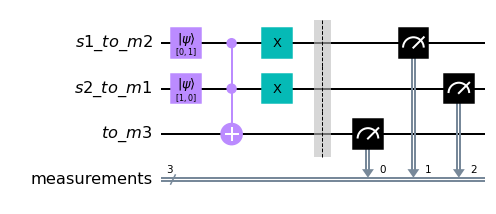
\includegraphics[width=0.85\linewidth]{./images/3qubit_qc.png}
	\caption{Circuit of the 3 Qubit Design}%
	\label{fig:3qubit_qc}%
\end{figure}

\textbf{Executing the circuits in both simulators and actual quantum computers:}
The codes are same as \hyperref[code:executing_the_quantum_circuit_on_a_simulator]{`Executing the Quantum Circuit on a Simulator'} and \hyperref[code:executing_the_quantum_circuit_on_a_quantum_computer]{`Executing the Quantum Circuit on an actual Quantum Computer'} section from the \hyperref[solution:1]{Approach 1}.

The result on the classical computer was exactly the same as the \hyperref[fig:5qubit_act]{previous result}. That on the Quantum Computer came out to be like \hyperref[fig:3qubit_act]{Figure 8}.

\begin{figure}[h]%
	\centering
	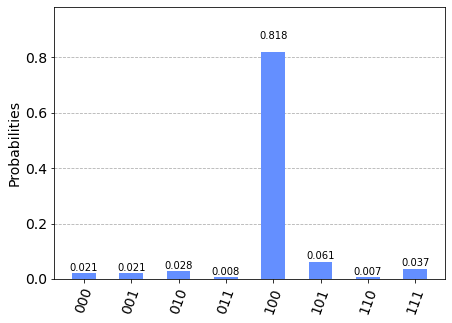
\includegraphics[width=0.85\linewidth]{./images/3qubit_act.png}
	\caption{\textbf{Histogram:} 3 Qubit Circuit executed on an actual Quantum Computer}%
	\label{fig:3qubit_act}%
\end{figure}